\documentclass[11pt]{ieeeconf}
\usepackage{graphicx}
\usepackage{float}
\usepackage{lettrine}
\usepackage{caption}



\newcommand\blfootnote[1]{%
  \begingroup
  \renewcommand\thefootnote{}\footnote{#1}%
  \addtocounter{footnote}{-1}%
  \endgroup
}

\title{Bumper Car Sumo}
\author{Jaden Simon - simonjaden223@gmail.com \\ \and
	   Melvin Bosnjak - meco0597@gmail.com \\ \and
	   Daniel Humeniuk - d.humeniuk@utah.edu \\ \and
	   http://bumpercarsumo.weebly.com/}

	   
\begin{document}

\maketitle

\begin{abstract}
Americans are not having fun anymore. The weight of capitalism is forcing families to work 60-hour weeks for low pay, leading to decreased enjoyment and productivity. An affordable and efficient form of entertainment would help solve this issue. In order to promote this, our group is designing a bumper car battle royale game. The project will have intuitive controls, simple yet fun mechanics, and a robust interface to allow for easy development. Continued play testing during development will allow us to monitor these objectives. Our ultimate goal is mutual enjoyment between us and our players.
\end{abstract}

\section{Introduction}
Entertainment is a fundamental part of the human experience. While some lucky few are able to derive satisfaction from their career, most people need something else to entertain themselves. This is the focus of our team's project: to develop an entertaining game with widespread appeal.

 The most important criteria of our game’s success are cost and entertainment efficiency. Our game must yield high levels of fun per minute played, while keeping costs as low as possible without compromising the entertainment value. Competition in games is a key element for high entertainment value \cite{vord:03}.  Because of this, our team decided to create a game where player-controlled robots attempt to push each other out of an arena. To facilitate gameplay, our robots need to be easily pushed around by other robots. Controls should be easy to enhance playability, though not too easy. We need a way to detect game conditions, such as when a robot is out of bounds or when a player wins. This could be done with a human referee, but that would take away immersion of the game. Because some players may not have friends to play with, it is desirable to have an AI to play against. 

Since cost is a contributing factor to our design, we will want to use existing technologies as much as possible. Robots can be constructed as a two-wheeled platform with wireless modules, similar to a Segway. They will be controlled through a web interface accessible by a wide variety of devices. Computer vision libraries will allow us to track the location of each robot if painted differently. Exact positioning solves the problem of detecting game conditions, plus giving us plenty of information to use for a basic AI. 

Our goal, above all else, is that our game is fun. Playtesting will be a major component of our design process, rethinking aspects of the game if it is not fun. Costs will be mitigated, but entertainment value will never be sacrificed for savings. Player enjoyment is our primary measure of success.

% Olliie bot figure
\begin{figure}[H]
\centering
\captionsetup{justification=centering}
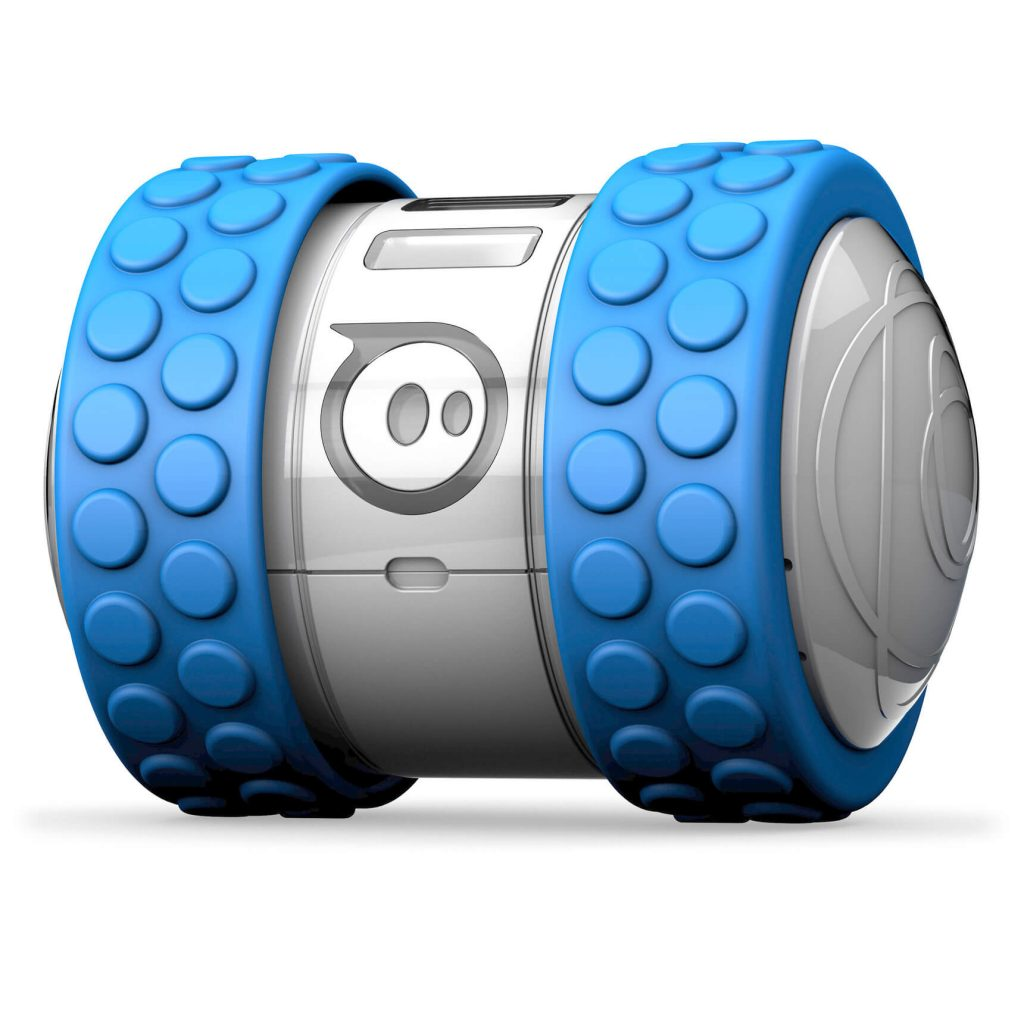
\includegraphics[width=0.5\textwidth]{images/SumoBot.png}
\caption{The Ollie from Sphero\\Source: Adapted from \cite{ollie:19}}
\label{Ollie}
\end{figure}

\section{Background}
The biggest component to our project is the robot. Two-wheeled wireless robots already exist and are mass produced, such as the Ollie (Fig \ref{Ollie}). While the Ollie has many of the features we require for our project, it does not give the level of control necessary to make our game a reality. On top of that, it is expensive at over \$80.00 per unit. The specifications for the Ollie are freely available online and will help guide us through the design of our own robots.


Tracking the robots would be a huge undertaking, but luckily there exists an open-source computer vision library called OpenCV. OpenCV provides algorithms to scan an image and identify desired patterns \cite{opencv:19}. With this, tracking can be done with only a camera, a computer, and a small bit of code. 

\section{Design}

To complete the project, we will need a main control mechanism (a hub), robots, controllers, and tracking. A centralized hub will be the core of the project, which will coordinate the other three components. The robots will use a custom PCB with an inertial measurement unit (IMU) and low-voltage motor driver, able to communicate via WiFi through an ESP8266. Our controllers will have both a physical and software interface. An overhead camera will be used to monitor the locations of our robots, which will be combined with IMU data for an extremely accurate positioning system. Separating these four components allows for simultaneous development by our team members.

\subsection{Hub}
% Talk more about AI 

The hub will be a Raspberry Pi device that will have four primary functions: To capture the game state from a camera peripheral, use computer vision to keep track of each robots location, host a web server that will have bi-directional communication with the controllers, and communicate wirelessly to relay the players' commands to their respective robots. Fig. \ref{Illustration} shows the basic illustration of the game. If time allows, then our AI implementation will be done on the hub. This component of the project requires no custom hardware and can be done entirely in software. Core hub software will take at most a month for full development and testing. 

% Game design figure
 \begin{figure*}[!t]
  \centering
  \captionsetup{justification=centering}
      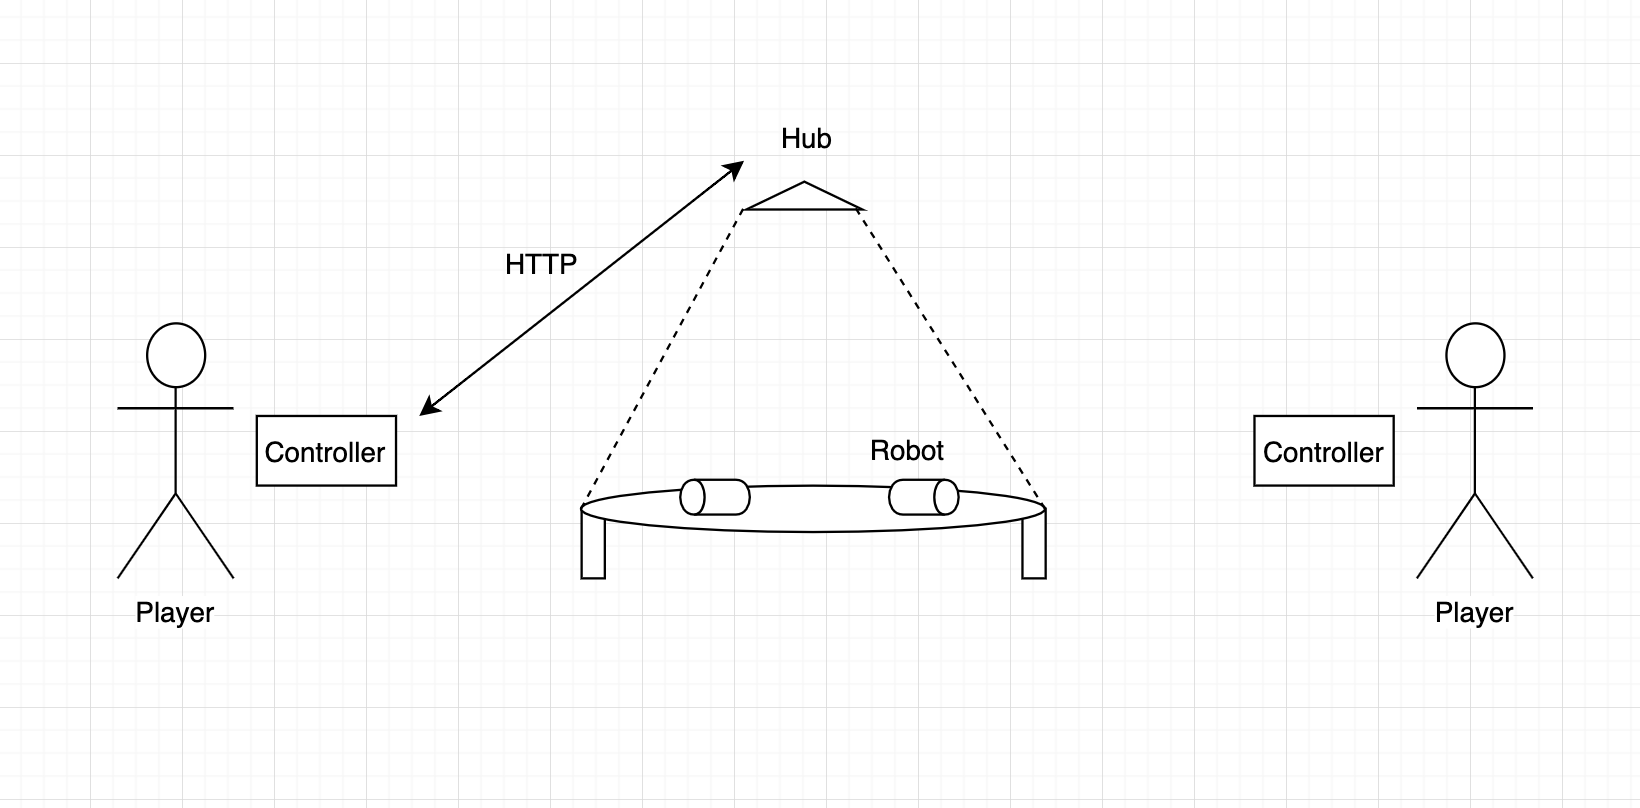
\includegraphics[width=14cm]{images/Overall.png}
        \caption{Overall game design}
        \label{Illustration}
\end{figure*}

\subsection{Robot}
% Describe in more detail 

Our robots will be cylindrically shaped with two wheels on each side of the body that can move in either direction (Fig. \ref{RobotFig}). In order to move forward, both of the wheels will spin at the same time at the same rate. To move backwards, the same principle applies in the opposite direction. Rotating the robot left or right requires spinning the motors in opposite directions. An ESP8266 microcontroller will provide WiFi and Bluetooth capability while also allowing for command interpretation from the hub. Our motors will require significant current so a custom driver will be required. The torque of our motors is important for our robots to be able to push each other around. Additional components can be added to keep track of orientation or acceleration. Batteries of suitable capacity and voltage will be determined once the robot requirements are finalized. The robot will take up to 3 months to fully develop and test due to its requirement of custom hardware. 

% Robot design figure
 \begin{figure}[H]
  \centering
      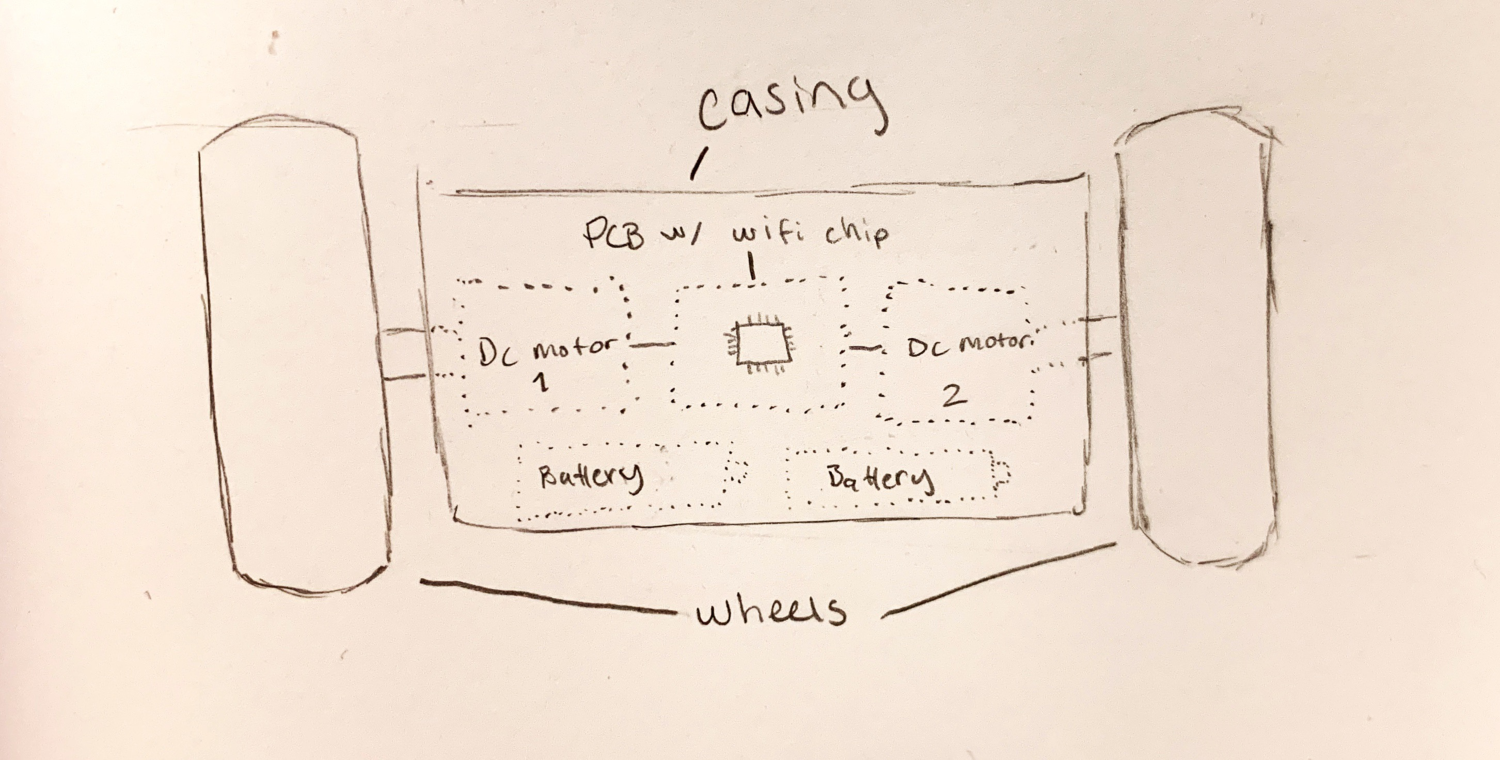
\includegraphics[width=0.5\textwidth]{images/RobotSketch.pdf}
        \caption{Basic robot layout}
        \label{RobotFig}
\end{figure}

\subsection{Controller}
% Talk about using Wii balance board and/or game console controller 
% Maybe talk about other ways to control the robots ? 
The controller provides the opportunity to add interesting game mechanisms that are unique to our game. We have been discussing ideas for unique control options and have come up with several ideas. The ideas discussed have been utilizing a web server in which players can use keyboard inputs to move the robots as they watch the game through the web camera. Another option is using existing technologies such as the Wii Balance board, as seen in Fig \ref{Wii}, or standard Super Nintendo Controllers which have the potential to be wireless. The last option is creating a custom controller with two foot pedals that drive separate motors on the robot. The final decision of the controller lies within how much it adds to the game play. Each controller will be discussed in further detail below.

% Wii fit board figure
\begin{figure}[H]
\centering
\captionsetup{justification=centering}
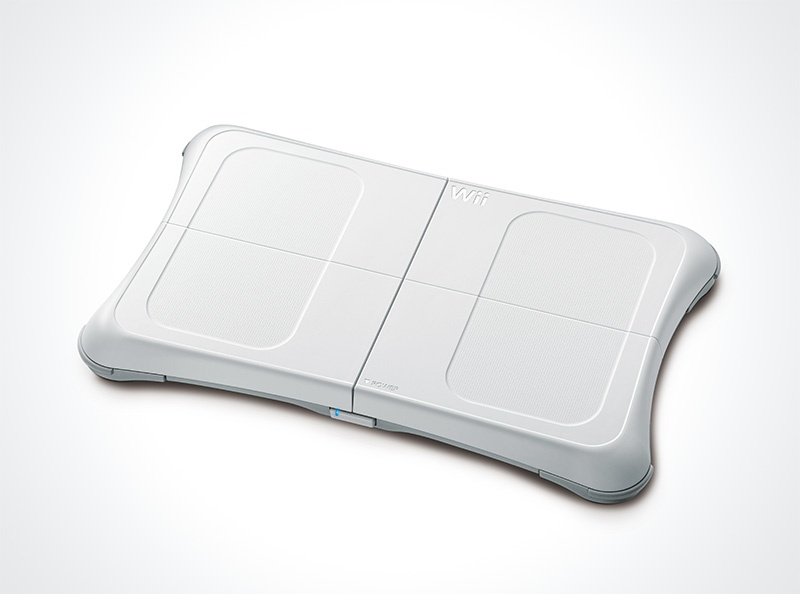
\includegraphics[width=0.5\textwidth]{images/wii.jpg}
\caption{The Wii Balance Board}
\label{Wii}
\end{figure}

A web-based control system will offer the cheapest possible controller with some possibilities to enhance the playing experience. The users will have the option to connect to a WiFi network and log into a website we will create for the game. The website will be streaming a live feed of the game play area via web camera technology. The players will receive a brief overview of the controls that are enabled on their keyboards and are then allowed to select a robot color of their choice. With the use of OpenCV, the robots will be tracked on screen with and player names will be displayed above their respective robot. This also adds potential to enhance the game with power-ups existing only in the cyber realm. The major draw back to this option is it will remove the players from the physical properties of the game. It is still possible for the players to enjoy the game as intended with controls on a laptop but this option does remain on the lower end of the selection process. 

The Wii Balance Board promises an interesting controller experience. 

We want our game to be easily accessible by a wide range of players. To achieve this we will use a combination of software and hardware controllers. Web applications can be run on numerous devices and are relatively easy to develop. Players would be able to access a web server on their own devices to control the robots. Our hub will act as the web server and process incoming commands, translating them into commands for the robots. The controller interface will be the arrow keys for a computer and buttons for a phone. Our web server may also send information about our robots back to the client, which may include orientation, speed, acceleration, or possibly a live camera feed. Basic user interface and web server software should only take two weeks.



\subsection{Tracking}

Tracking will be done by the hub using a camera and OpenCV. The casings for each robot will be designed in such a way to allow for easy identification by algorithms. Players who leave the camera's field of view will be considered eliminated by the hub, preventing control of the robot by the player. Since our camera will be static, the total play area is limited by our camera's height and field of view. Our play surface will be monochromatic which increases our tracking capability, though we should be able to track with an arbitrary surface. The timeline for tracking is largely dependent on the hub and the robot, though 2 weeks seems like a reasonable amount of time.

\section{Game Mechanics}

\subsection{Game Modes}

There will be many game modes to select from. The primarily plan was to design the game arena to accommodate only one game mode. The team has elected to enable for multiple game modes to provide longevity to the product.    

\section{Timeline}
% Every person needs at least 5 milestones 

In order to finish our project before demo day, we have created a timeline. While the deadlines listed here are not set in stone, it should give us a good idea of what we need done by when. The length of the bars represent about how long it should take to complete the task. Each group member is assigned to a certain task dependent on the bar's color, though there is some flexibility there as well. Some of the tasks are dependent on the completion of previous tasks, so it is important for us not to get too far behind schedule. 

\subsection{Spring}
For the remaining month of May we will finalize our required parts list. This includes verifying we have the correct parts, checking availability, and price calculations.

\subsection{Summer}
The summer will consist of ordering and gathering the resources needed as well as detailed design for each component of the project. Basic documentation of our hardware and software interfaces will be completed by the end of the summer. We will complete a basic software interface and start experimenting with hardware interfaces. If time allows then we can create a basic play surface, since it is not dependent on the completion of any singular component.

\subsection{Fall}
Most of the legwork for the project will be done during the fall. With all components gathered and the design completed all that will be left to do is to assemble, test, and finalize documentation. Each project component will be worked on simultaneously. Integration between the four components of the project will not take long if our interfaces were designed correctly, perhaps only a week or two. The minimum requirements of the project is planned to be completed and tested a month before the demo day. A large amount of extra time allows us to experiment with additional features that will hopefully add to the entertainment value.

\subsection{Component Assignments}
As already discussed, the project is separated into 4 key components. Each component will have a single group member act as lead developer. Robots and tracking will be managed by Jaden. Development of the hub and its communication protocol will be done by Melvin. Dan is tasked with creating the software controller interface as well as working on variations of hardware interfaces. 

\section{Resources}
% Flesh out this section (full BOM) 
% Part number, lead time, unit cost, quantity, form factor, etc.
\subsection{Bill of Materials}

Each robot will require 2 DC motors with wheels, several batteries, a PCB that includes an ESP8266 microcontroller and motor drivers for each DC motor, and a casing to enclose and protect the internals. The casing will be designed and 3d printed by our group. Various ICs and small electrical components will be required based off our circuit designs. The design, testing, and implementation of the robot will take the bulk of the time required for this project.

A Raspberry Pi will act as the hub, handling all game mechanics and user-robot interactions. The Raspberry Pi 3 Model B+ has a quad core 1.4GHz processor which should be enough processing power for these tasks. Tracking is a fundamental component of the hub and will require a camera, ideally with high resolution and FPS. The options for the camera are the Raspberry Pi camera and the Logitech C922x Pro Stream Webcam. Software on the hub will depend on multiple open source libraries to function, though will still require significant custom software to operate.

The playing field will be constructed out of a simple table top with some 2 x 4's to hoist up the camera, with power and data cables running down to connect to the hub.

\subsection{Vendor List}
% List all vendors with contact information 

\section{Group Logistics}
In order to stay on top of our set deadlines, our group will be meeting at least once a week to discuss current tasks, issues we have experienced, and new ideas for our game. These meetings are logged on our website. Because Melvin will be in Idaho for the duration of the summer, our meetings will have to be digital and infrequent. In the fall we will resume the weekly meetings.

\section{Risk Management}
% Describe risks for each task, some might not have any 

\section{Testing}
Much of our time spent testing will be focused on robot design and user experience. The most complicated part of our robot will be the integration of a battery, but once that is complete we will focus on debugging software communication protocols. In addition, play-testing of the project is fundamental to our success. We must ensure that our game is entertaining through repeated testing of robot collisions and the user interface. Collisions with robots should feel powerful and the user interface should be responsive and free of frustration. Beyond that, we will need to experiment with the durability of our robots to make sure they do not break during play.

\section{Project Demo}
% Describe what will be highlighted in the demo 

On demo day, we hope to achieve a minimum requirement of 4 robots, basic user interface, and a single game mode. While 4 robots will provide enough competition to be entertaining, we ideally want 8 robots to allow more people to play. Basic user interface would only have options to control the robots in the 4 cardinal directions. More game modes are simple to implement but add enormous entertainment value.

\subsection{Setup}
First players connect to our web server through a device of their choice. Connections made in previous rounds will be preserved. Players then choose an available robot to play as. Each selected robot must be placed in designated spots, which will have to be done by humans. Once the hub detects that all robots are in the play area, the game can begin. 

\subsection{Game Round}
Each game round will depend on the game mode. In all of our game modes, players are eliminated if their robot leaves the play area. For a free-for-all, the game round ends when all but one player is eliminated. If a team mode is implemented, then a game round ends when only a single team remains. Game modes may have time limits, though this will depend on play testing during development.

\subsection{Post Game}
If we are able to meet our minimum requirements, then additional features will be added to aid user experience. This would include post game reports that contain information about the player such as eliminations, maximum speed, or the biggest hit taken. After any post game reports, our demo will start again at the setup.

\section{Project Status}
% Current status of our project
% Robot PCB pretty much

\section{Conclusion}
% Summarize entire proposal, include lessons learned so far (management/team/engineering) 
% Include biggest risks, analyze task dependency 
% Final advertisement of project 

\bibliographystyle{IEEEtran}
\bibliography{IEEEabrv,bib/ref}

\end{document}